\documentclass[compress, aspectratio=169]{beamer}
%\setbeameroption{show notes on second screen=left}
\usepackage[utf8]{inputenc}
\usepackage{braket}
\newcommand{\identity}[0]{\mathbf{1}}
\newcommand{\Op}[1]{\ensuremath{\mathsf{\hat{#1}}}}
\newcommand{\TildeOp}[1]{\ensuremath{\mathsf{\tilde{#1}}}}
\newcommand{\Abs}[1]{\left|#1\right|}
\newcommand{\AbsSq}[1]{\left|#1\right|^2}
\newcommand{\Norm}[1]{\left\lVert#1\right\rVert}
\newcommand{\NormSq}[1]{\Norm{#1}^2}
\newcommand{\tr}{\mathsf{tr}}
\newcommand{\Tr}{\mathsf{tr}}
\newcommand{\SU}{\ensuremath{\text{SU}}}
\newcommand{\ketbra}[2]{\ket{#1}\!\bra{#2}}
\newcommand{\mirror}{\text{mirror}}
\newcommand{\tgt}{\text{tgt}}
\newcommand{\pop}{\operatorname{pop}}
\newcommand{\dd}{\mathsf{d}}
\newcommand{\ii}{\mathsf{i}}
\newcommand{\Integers}{\mathbb{Z}}
\renewcommand{\Re}{\mathsf{Re}}
\renewcommand{\Im}{\mathsf{Im}}
\newcommand{\partdifquo}[2][{}]{\frac{\partial #1}{\partial #2}}
\newcommand{\Complex}{\mathbb{C}}
\newcommand{\Liouvillian}{\mathcal{L}}
\usepackage{textcomp} % provides \textmu
\usepackage{tikz,pgflibraryshapes}
\usepackage{hyperref}
\usepackage{fontawesome}
\usetikzlibrary{arrows.meta, calc, decorations.pathmorphing, backgrounds, positioning}

%% Notes on screenshots:
%
% - Make sure ``Reduce Transparency'' in the Accessibility settings (Display) is off
% - Size window to 1270 x 625 (2540 x 1250 retina)
%   - if no title on slide: increase height +41 to 666  (1332 retina)
% - Take screenshots at retina resolution
% - Terminal (iTerm) is at standard size +5 font size increases
% - JupyterLab in Arc – for slide without title:
%   - total window size 1364 x 800
%   - ``Simple Interface'' (View Menu)
%   - ``Presentation Mode'' (View Menu)
%   - No status bar (View Menu)


\input{arlwide_theme/theme.tex}

\title{Quantum Dynamics and Control\\ with QuantumControl.jl}
\author[Michael Goerz~\raisebox{0.75pt}{\tikz \fill (0,0) circle (0.75pt);}~\raisebox{-1.4pt}{\includegraphics{images/mastodon}}\kern-0.5pt\href{https://qubit-social.xyz/@goerz}{goerz@qubit-social.xyz}]{Michael~H.~Goerz}
\institute[Army Research Lab]{DEVCOM Army Research Lab}
\date{JuliaCon 2023}

\begin{document}

{%  Title page
  \setbeamertemplate{footline}{}
  \frame{%
    \titlepage
    \note{\dots}
  }
}
\addtocounter{framenumber}{-1}

\begin{frame}{JuliaQuantumControl}
  \begin{textblock}{15.5}(0.25,1.00)
    \includegraphics<1>[width=\textwidth]{images/JuliaQuantumControl}
    \includegraphics<2>[width=\textwidth]{images/JuliaQuantumControlPackages}
    \includegraphics<3>[width=\textwidth]{images/JuliaQuantumControlPackages_1}
    \includegraphics<4>[width=\textwidth]{images/JuliaQuantumControlPackages_2}
  \end{textblock}
  \note<1>{%
    Alright, so I wanna talk about the work we are doing to implement quantum optimal control in the JuliaQuantumControl organization
  }
  \note<2>{which has the \dots}
  \note<3>{\dots QuantumControl package as a high-level framework, and as part of that the \dots}
  \note<4>{\dots QuantumPropagators package to simulate quantum dynamics.}
\end{frame}

\begin{frame}{What is Quantum Control?}
  \begin{center}
    \Large \bf \color{DarkRed} Steer a quantum system in some desired way
  \end{center}
  \note<1>{%
    So what is quantum control?

    Well, it's basically the question of how to \emph{actively steer} a quantum system in some desired way
  }
\end{frame}

\begin{frame}{Quantum Gates}
  \begin{textblock}{15.5}(0.25,1.00)
    \includegraphics<1>[width=\textwidth]{images/YaoCircuit}
    \includegraphics<2>[width=\textwidth]{images/YaoCircuit_hl}
  \end{textblock}
  \note<1>{%
    So I think a lot of you are coming from a quantum computing background

    So usually you're working at the level of a circuit diagram like this from the Yao documentation,

    or you have packages like Qiskit or Braket.

    But now from a control perspective we're interested in how exactly you would implement one of these gates physically, like \dots
  }
  \note<2>{%
    \dots this controlled rotation.

    So in Qiskit at least, in the last couple of years they've added what they call ``pulse-level control'', so that's what we're talking about here.


    And this really goes to the \emph{physics} of your platform
  }
\end{frame}

\begin{frame}{Two-Transmon Gate}
  \begin{textblock}{7.5}(0.5,1.25)
    \includegraphics[width=\textwidth]{images/coupled_transmon}\\
    \hfill\tiny{Majer \emph{et al.} Nature 449, 443 (2007)}\hspace{2mm}~\\
  \end{textblock}
  \begin{textblock}{6}(9,2.25)
    \begin{equation*}
      \Op{H} = \Op{H}_0 + \epsilon(t) \Op{H}_1
    \end{equation*}
  \end{textblock}
  \begin{textblock}{5}(9.5,3.2)
    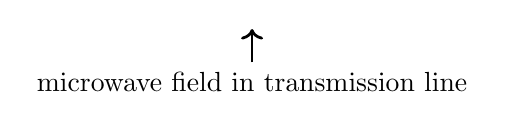
\begin{tikzpicture}
      \draw[->, line width = 1pt] (0, 0) -- +(0, 12pt);
      \node[below] (0,0) {microwave field in transmission line};
    \end{tikzpicture}
  \end{textblock}
  \begin{textblock}{4}(3,5.5)
    \includegraphics<2->[height=3cm]{images/YaoCircuit_cutout}
  \end{textblock}
  \begin{textblock}{10}(6,6.0)
    \onslide<2->{%
      \begin{equation*}
        \left.\begin{aligned}
        \ket{00} & \rightarrow \text{CR}_2 \ket{00} \\
        \ket{01} & \rightarrow \text{CR}_2 \ket{01} \\
        \ket{10} & \rightarrow \text{CR}_2 \ket{10} \\
        \ket{11} & \rightarrow \text{CR}_2 \ket{11}
        \end{aligned} \quad \right\} \quad \begin{aligned}
          & \text{with the same}~\epsilon(t); \\
          & \text{acting on logical subspace}
        \end{aligned}
      \end{equation*}
    }
  \end{textblock}
  \note<1>{%

    So, for example, if you have superconducting qubits you'd have something like this Transmon circuit,

    where you have two transmons with a shared transmission line, and the control you have is the field that you put into the transmission line.
  }
  \note<2>{%
    And now we're going to try to find a field so that every logical basis state for a two-qubit system evolves so that it implements this controlled rotation.

    \dots

    But there's other control problems besides implementing gates.
  }
\end{frame}


%\begin{frame}{Charting the circuit QED design landscape using optimal control}
%  \begin{textblock}{15}(0.5,1.5)
%    \begin{itemize}
%      \item Scan over transmon and cavity frequencies
%      \item At each point: optimize for entangling gate and universal set of single-qubit gates
%      \item Identify optimal quasi-dispersive straddling qutrit regime (``QuaDiSQ'')\\
%            for fast gates $\sim 10$\,ns
%    \end{itemize}
%  \end{textblock}
%  \begin{textblock}{15}(0.5,4.25)
%    \includegraphics[width=\textwidth]{images/transmon_landscape}\\
%    \hfill \footnotesize{Goerz \emph{et al.} npj Quantum Information 3, 37 (2017)}
%  \end{textblock}
%\end{frame}


\begin{frame}{Controlling the transport of an ion}
  \begin{textblock}{7.5}(0.5,1.5)
    \includegraphics[width=0.95\textwidth]{images/FuerstNJP2014_trap}\\
    \footnotesize{Fürst \emph{et al.} New J. Phys. 16, 075007 (2014)}
  \end{textblock}
  \begin{textblock}{4}(10.0,2.5)
    {\color{DarkRed}
      Find electrode voltages \\
      to move trapped ions
    }
  \end{textblock}
  \begin{textblock}{7.5}(8.5,4.5)
    \onslide<2>{%
      \includegraphics[width=0.8\textwidth]{images/BruzewiczNPJQI2019_Fig1}\\
      \tiny{Bruzewicz \emph{et al.}  npj Quantum Inf 5, 102 (2019)}
    }
  \end{textblock}
  \note<1>{%
    For example, if you have ions in a segmented trap, you might want to move them over some distance,

    and then the control is the voltage that's applied to every one of these segments to sort of create a trap potential that moves this ion along
  }
  \note<2>{%
    And you could build that into some kind of complex shuffling of atoms on a 2D chip.
  }
\end{frame}


\begin{frame}{Tractor atom interferometry}
  \begin{textblock}{8.5}(0.75,1.5)
    \includegraphics[width=\textwidth]{images/RaithelQST2022_Fig4}\\
    \footnotesize{Raithel \emph{et al.} Quantum Sci. Technol. 8, 014001 (2022)}
  \end{textblock}
  \begin{textblock}{6}(9.75,3.5)
    {\color{DarkRed}
      Find non-adiabatic tractor potential\\
      closing interferometric path
    }
  \end{textblock}
  \note<1>{%
    Or, something that's closer to what I'm doing these days,

    you could have some trapped atoms where you split them into two trapping potentials and then you move the potentials along two different pathways to implement an interferometer.

    And then you have to find exactly the right trajectory to combined the wavepackets again at the end.
  }
\end{frame}


\begin{frame}{Fortran: QDYN library}
  \begin{textblock}{15.5}(0.25,1.00)
    \includegraphics[width=\textwidth]{images/qdyn}
  \end{textblock}
  \begin{textblock}{3.5}(11.05,3.0)
    \begin{center}
      \bf
      C.~Koch group\\
      FU Berlin
    \end{center}
  \end{textblock}
  \note<1>{%
    So traditionally we've done this with Fortran,

    for example with this QDYN library that I was the maintainer of during my PhD.

    And Fortran is really a very nice language for the kind of numerics you have to do here.

    But there's two problems with Fortran.

    One is just the workflow. So you end up writing Python scripts to do your modeling and then you write out data and config files to disk, and the then you run your Fortran program, and you do you analysis, and there's just a lot of overhead with managing all of that.

    And the other problem is flexibility. So once you have a big library, if you want to do something new that doesn't really quite fit into your existing data structures, things get just more and more sprawling and complicated.

    So you might start out with just basic energy levels like for the transmon, but then you also want to do molecular dynamics, or rotations, or spin systems

    and then you have to manage all these different data structures and code paths.
  }
\end{frame}


\begin{frame}{Python}
  \begin{textblock}{15.5}(0.25,1.00)
    \includegraphics[width=\textwidth]{images/python_krotov}
  \end{textblock}
  \begin{textblock}{6}(1.2,7.8)
    \footnotesize{Goerz \emph{et al.} SciPost Phys. 7, 80 (2019)}
  \end{textblock}
  \note<1>{%
    So we also tried to port some of these optimization methods to Python.

    And that works pretty well for the optimization as such,

    and it definitely makes the workflow a lot easier,

    but for the underlying simulation of quantum dynamics the performance just isn't there.

    And on top of that, Python's GIL really kills any kind of parallelization.

    So then you have to start doing something like Cython, which just gets very technical to write and to package in a very annoying way,

    and on top of that neither Python or C really have very good semantics for the kind of numerics that we want to do.
  }
\end{frame}


\begin{frame}
  \begin{center}
    {\Large \color{DarkRed} \bf Why Julia?}
    \vspace{1.5cm}
    \pause
    \begin{itemize}
      \item Flexibility \pause
      \item Performance \pause
      \item Expressiveness
    \end{itemize}
  \end{center}
  \note<1>{%
    So why Julia then?
  }
  \note<2>{%
    So the first aspect is flexibility.

    So compared to Fortran, you have a much nicer workflow in notebooks,

    but you also have multiple dispatch to solve that problem that you want to do sort of unusual things with custom data structures

    So we can just separate that extremely well in Julia.
  }
  \note<3>{%
    And then of course the second aspect is performance, compared to Python.

    And that really becomes relevant for open systems or noisy systems, where an optimization might run for several weeks on a cluster, which really isn't something you can do in Python.
  }
  \note<4>{%
    And then last, but not least, Julia also has an amazing expressiveness compared to both Fortran and Python, with a real focus on linear algebra and unicode, and things like multiple dispatch
  }
\end{frame}


\begin{frame}{QuantumControl.jl examples}
  \begin{textblock}{15.5}(0.25,1.00)
    \includegraphics[width=\textwidth]{images/example_docs}
  \end{textblock}
  \note<1>{%
    Ok, so let's just jump in to an example.

    So this is something that I've adapted from one of the examples in the documentation,

    and I'll go into some of the details and design principles of the QuantumControl package as we go along.
  }
\end{frame}


\begin{frame}
  \begin{textblock}{15.5}(0.25,0.5)
    \includegraphics<1>[width=\textwidth]{images/example/01} % still image
    \includegraphics<2>[width=\textwidth]{images/example/01}
    \includegraphics<3>[width=\textwidth]{images/example/02}
    \includegraphics<4>[width=\textwidth]{images/example/03}
    \includegraphics<5>[width=\textwidth]{images/example/04}
    \includegraphics<6>[width=\textwidth]{images/example/05}
    \includegraphics<7>[width=\textwidth]{images/example/06}
    \includegraphics<8>[width=\textwidth]{images/example/07}
    \includegraphics<9>[width=\textwidth]{images/example/08}
    \includegraphics<10>[width=\textwidth]{images/example/09}
    \includegraphics<11>[width=\textwidth]{images/example/10}
    \includegraphics<12>[width=\textwidth]{images/example/11}
    \includegraphics<13>[width=\textwidth]{images/example/12}
    \includegraphics<14>[width=\textwidth]{images/example/13}
    \includegraphics<15>[width=\textwidth]{images/example/14}
  \end{textblock}
  \note<1>{%
    So the example is going to be the same one that I talked about before, which is these two superconducting transmon qubits coupled to a shared transmission line.
  }
  \note<2>{%
    (01)\par
    And just for simplicity, we're going to assume that we're in what's called the dispersive limit, where the coupling between the qubit and the cavity is relatively small, so that you can adiabatically eliminate the cavity.
  }
  \note<3>{%
    (02)\par
    and what you end up with is that the microwave field that you put in the cavity here\dots
  }
  \note<4>{%
    (03)\par
    \dots ends up effectively driving the transitions of the qubit\dots
  }
  \note<5>{%
    (04)\par
    and then you also have a static qubit-qubit interaction between the two qubits
  }
  \note<6>{%
    (05)\par
    So the energies of the qubits are going to be on the order of GHz with a timescale of nanoseconds
  }
  \note<7>{%
    (06)\par
    And we're going to truncate the levels of this qubit to 6 levels
  }
  \note<8>{%
    (07)\par
    So that means that the dimension of the total Hilbert space is going to be 36, which is not too big, but also not completely trivial.
  }
  \note<9>{%
    (08)\par
    Okay, and now we can write out the Hamiltonian\dots
  }
  \note<10>{%
    (09)\par
    And the first thing we're going to do is to go to a rotating frame, which means that we shift the qubit frequencies down by the driving frequency.

    The other thing that that does is to make the control field complex, where the phase of the field gives you the deviation from the drive frequency.
  }
  \note<11>{%
    (10)\par
    Well, and beyond that we can now just write out the Hamiltonian very straightforwardly...
  }
  \note<12>{%
    (11)\par
    So we have this anharmonic Duffing oscillator for the two transmons here and here...
  }
  \note<13>{%
    (12)\par
    And then we have the static interaction term here.
  }
  \note<14>{%
    (13)\par
    And for the control term we want to treat the real part and the imaginary part of the control as two independent control fields, so we split that into two terms
  }
  \note<15>{%
    (14)\par
    So let me just talk about this "hamiltonian" function\dots
  }
\end{frame}


\begin{frame}{Dynamical Generator}
  \begin{textblock}{15.5}(0.25,1.00)
    \includegraphics<1>[width=\textwidth]{images/generator_glossary}
    \includegraphics<2>[width=\textwidth]{images/generator_glossary_g2}
    \includegraphics<3>[width=\textwidth]{images/generator_glossary_g3}
    \includegraphics<4>[width=\textwidth]{images/generator_glossary}
    \includegraphics<5>[width=\textwidth]{images/generator_glossary_g2}
    \includegraphics<6>[width=\textwidth]{images/generator_glossary}
    \includegraphics<7>[width=\textwidth]{images/generator_glossary_g1}
  \end{textblock}
  \begin{textblock}{15.5}(0.25,4.80)
    \begin{center}
      \includegraphics<5>[width=11.55cm]{images/hamiltonian_call}
    \end{center}
  \end{textblock}
  \note<1>{%
    So the underlying concept that's pretty central in the QuantumControl package is that of a ``dynamical generator''

    which is the object that describes the dynamics of a state

    so a time-dependent Hamiltonian or Liouvillian

    and mathematically the structure that's most directly supported is \dots
  }
  \note<2>{%
    \dots this equation here,

    where you have a drift term, and then you have control operators that get multiplied with a control amplitude

    And the control amplitude depends on one or more control functions epsilon, which are what we're going to be manipulating directly with optimal control.

    So in many cases, the control amplitude is just directly the control function, and then you get \dots
  }
  \note<3>{%

    this linear control Hamiltonian down here

  }
  \note<4>{%

    But in general you could have an amplitude where you add noise on top of your control function, or you have some amplitude that depends non-linearly on one or more controls, like a spin-orbit coupling that's quadratic in the field, or you have some transfer function of a waveform generator, or so many other things.

    So it's really quite flexible.
  }
  \note<5>{%
    And the call to ``hamiltonian'' gives you exactly this structure, where you give tuples of control operators and control amplitudes
  }
  \note<6>{%
    But you could in fact be even more general\dots
  }
  \note<7>{%
    \dots and have operators that depend in some completely arbitrary way on any number of control functions
  }
\end{frame}


\begin{frame}{Generator Interface}
  \begin{textblock}{15.5}(0.25,1.00)
    \includegraphics<1>[width=\textwidth]{images/generator_interface}
    \includegraphics<2>[width=\textwidth]{images/generator_interface_get_controls}
    \includegraphics<3>[width=\textwidth]{images/generator_interface_evaluate}
  \end{textblock}
  \note<1>{%
    So ultimately we just have an abstract interface for what you can use as a dynamical generator

    So you have to be able to \dots
  }
  \note<2>{%
    \dots extract ``controls'', which are scalar functions or arrays, because otherwise you don't have anything to do optimal control on

    And you have to be able to \dots
  }
  \note<3>{%
    \dots evaluate your generator by plugging in values for the controls at a particular point in time

    and that has to give you an ``operator''

    which has its own abstract interface

    but that's basically just an object for which you have to define all the linear algebra operations that you can multiply it to a state.
  }
\end{frame}

\begin{frame}{QuantumControl.jl is not a modeling framework!}
  \begin{textblock}{15.5}(0.25,1.00)
    \includegraphics<2>[width=\textwidth]{images/quantumoptics}
  \end{textblock}
  \note<1>{%
    So an important take-away is that the QuantumControl package is not a modeling framework
  }
  \note<2>{%
    So in something like QuantumOptics.jl you have data structures that are specific to the \emph{physics} of the problem, with, like, position or momentum operators, or Gaussian states, or anything like that.

    So you're not going to have anything like that in the QuantumControl package.

    But the idea would be that you can take data structures from QuantumOptics, or maybe something like matrix-product-states, or anything else like that, and use them as components of the dynamical generator in QuantumControl together with control functions.
  }
\end{frame}


\begin{frame}
  \begin{textblock}{15.5}(0.25,0.5)
    \includegraphics<1>[width=\textwidth]{images/example/15}  % still image
    \includegraphics<2>[width=\textwidth]{images/example/15}
    \includegraphics<3>[width=\textwidth]{images/example/16}
    \includegraphics<4>[width=\textwidth]{images/example/17}
    \includegraphics<5>[width=\textwidth]{images/example/18}
    \includegraphics<6>[width=\textwidth]{images/example/19}
    \includegraphics<7>[width=\textwidth]{images/example/20}
    \includegraphics<8>[width=\textwidth]{images/example/21}
    \includegraphics<9>[width=\textwidth]{images/example/22}
    \includegraphics<10>[width=\textwidth]{images/example/23}
    \includegraphics<11>[width=\textwidth]{images/example/24}
    \includegraphics<12>[width=\textwidth]{images/example/25}
  \end{textblock}
  \note<1>{%
    So let's get back to the example\dots
  }
  \note<2>{%
    (15)\par
    \dots and talk about the initial guess for the driving field.
  }
  \note<3>{%
    (16)\par
    So this is going to be an example for what we just talked about -- the distinction between a control amplitude and a control field.

    So physically what we want to have as a control amplitude is something that switches on from zero to 35 MHz, and then stays constant for about 400 ns and switches down again.

    And we're going to separate that into a shape that's going to stay fixed that just goes from zero to one and then stays one and goes down again

    And then we're going to multiply that with an arbitrary control function,...
  }
  \note<4>{%
    (17)\par
    ... and initially that control function is just going to be a constant 35 MHz.

    And we're also going to assume that we're at the driving frequency, which means ...
  }
  \note<5>{%
    (18)\par
    ...the imaginary part is going to be initially zero.
  }
  \note<6>{%
    (19)\par
    Okay, so we can instantiate that,

    and now if we plot it, we can see that is exactly what I just described.
  }
  \note<7>{%
    (20)\par
    And now we can instantiate the Hamiltonian based on that.
  }
  \note<8>{%
    (21)\par
    So for the states, we have a logical subspace of the two lowest levels for each of the two qubits, and then additional levels on top of that
  }
  \note<9>{%
    (22)\par
    And we'll tensor that into a logical basis for the two-qubit system
  }
  \note<10>{%
    (23)\par
    And we if we look at just one of the states, we'll see that it's a 36 dimensional vector, with a one in one particular place and zero everywhere else
  }
  \note<11>{%
    (24)\par
    Okay, so let's look at the dynamics of the system
  }
  \note<12>{%
    (25)\par
    So we're going to use this propagate function, and this function is there to simulate the time dynamics...
  }
\end{frame}

\begin{frame}{QuantumPropagators.jl}
  \begin{textblock}{6.5}(0.5,1.00)
    \includegraphics<1>{images/pulse_examples_simple}
    \includegraphics<2>{images/pulse_examples_continuous}
    \includegraphics<3>{images/pulse_examples_discrete}
    \includegraphics<4->{images/pulse_examples_pwc}
  \end{textblock}
  \begin{textblock}{7}(8.25,1.00)
    \begingroup
      \addtolength{\jot}{1em}  % increase space between rows
      \begin{align*}
        i \hbar \frac{\partial}{\partial t} \ket{\Psi(t)} &= \Op{H}(\{\epsilon_l(t)\}) \ket{\Psi(t)}\\
        i \hbar \frac{\partial}{\partial t} \hat\rho(t) &= \Liouvillian(\{\epsilon_l(t)\})[\hat\rho(t)]
      \end{align*}
    \endgroup
    %\begin{equation*}
      %\Op{H} = \Op{H}_0 + \Omega_{\Re}(t) \Op{H}_{1}^{(\Re)} + \Omega_{\Im}(t) \Op{H}_{1}^{(\Im)}
    %\end{equation*}
  \end{textblock}
  \begin{textblock}{14}(1.0,4.45)
    \onslide<5->{%
      \begin{center}
        PWC propagator: {\color{DarkRed}$\Op{U}_n = \exp[-\frac{i}{\hbar} \Op{H}_n dt]$} for $n$'th time slice
      \end{center}
    }
  \end{textblock}
  \begin{textblock}{14}(1.0,5.95)
    \onslide<6->{%
      $\Rightarrow$ evaluate $\Op{U}_n \ket{\Psi}$ (or $\mathcal{U}_n[\hat\rho]$) as a polynomial expansion
      \vspace{5mm}
      \onslide<7->{
        \begin{itemize}
          \item Hermitian Hamiltonian $\rightarrow$ Chebychev polynomials
          \item Non-Hermitian Hamiltonian or Liouvillian $\rightarrow$ Newton polynomials
        \end{itemize}
      }
    }
  \end{textblock}
  \note<1>{%
    \dots for the Schrödinger equation, or the Liouville equation for an open system,
    with some number of control fields epsilon-ell

    So why not just throw this into DifferentialEquations or use the dynamics from QuantumOptics or something like that?

    So remember that we're going to \dots
  }
  \note<2>{%
    \dots \emph{change} the control fields with optimal control.

    And if you want to the control procedure to produce arbitrary fields, you pretty much have to \dots
  }
  \note<3>{%
    \dots \emph{discretize} them to some time grid.

    And then the standard thing to do is to take the controls as \dots
  }
  \note<4>{%
    \dots piecewise constant on that time grid.

    And then the optimal control will tune the values at the different time slices.
  }
  \note<5>{%
    So now you don't actually have to solve this as a differential equation,

    but you know that the propagator for on time slice is just e to the minus i-H-dt.
  }
  \note<6>{%
    And you can just \emph{evaluate} that by expanding the application of that propagator into a polynomial expansion.

    So think Taylor series, but in fact the Taylor series is a particularly badly converging polynomial series,
  }
  \note<7>{%
    So instead you can use Chebychev polynomials if the generator only has real eigenvalues

    Or Newton polynomials for example for open quantum systems.
  }
\end{frame}

\begin{frame}{Propagator Interface}
  \begin{textblock}{15.5}(0.25,1.00)
    \includegraphics[width=\textwidth]{images/propagator_interface}
  \end{textblock}
  \note<1>{%
    And again this is all implemented via an abstract interface.

    So you can implement propagators where you just need an init-prop function

    And then you can step through the time grid with a prop-step function

    So the Schrödinger equation is implicit in this propagator, but you have have something different like a Gross-Pitaevskii equation, you could define your own propagator according to that interface.
  }
\end{frame}


\begin{frame}
  \begin{textblock}{15.5}(0.25,0.5)
    \includegraphics<1>[width=\textwidth]{images/example/26} % still image
    \includegraphics<2>[width=\textwidth]{images/example/26}
    \includegraphics<3>[width=\textwidth]{images/example/27}
    \includegraphics<4>[width=\textwidth]{images/example/28}
    \includegraphics<5>[width=\textwidth]{images/example/29}
    \includegraphics<6>[width=\textwidth]{images/example/30}
    \includegraphics<7>[width=\textwidth]{images/example/31}
    \includegraphics<8>[width=\textwidth]{images/example/32}
    \includegraphics<9>[width=\textwidth]{images/example/33}
    \includegraphics<10>[width=\textwidth]{images/example/34}
    \includegraphics<11>[width=\textwidth]{images/example/35}
    \includegraphics<12>[width=\textwidth]{images/example/36}
    \includegraphics<13>[width=\textwidth]{images/example/37}
    \includegraphics<14>[width=\textwidth]{images/example/38}
    \includegraphics<15>[width=\textwidth]{images/example/39}
    \includegraphics<16>[width=\textwidth]{images/example/40}
    \includegraphics<17>[width=\textwidth]{images/example/41}
    \includegraphics<18>[width=\textwidth]{images/example/42}
  \end{textblock}
  \note<1>{%
    Ok, so let's get back\dots
  }
  \note<2>{%
    (26)\par
    So we're going to be interested in what happens with this system in the logical subspace
  }
  \note<3>{%
    (27)\par
    So we're going define this "observable" where we take the overlap with every one of the logical basis states.
  }
  \note<4>{%
    (28)\par
    And if we do that for propagating all of the basis states,

    because we have this parameter "storage equals to true",
  }
  \note<5>{%
    (29)\par
    just for one of them, it's going to be a matrix of these complex projections at every point in time
  }
  \note<6>{%
    (30)\par
    And we can concatenate that to get a 4 by 4 matrix, so that's the gate in the logical subspace, at every point in time.
  }
  \note<7>{%
    (31)\par
    Well, and in order to analyze that, we going to use something called the "gate concurrence"

    And the "gate concurrence" is just a measure of how much entanglement you can get if you apply the gate to some specific separable input state.
  }
  \note<8>{%
    (32)\par
    So probably the most well-known gate that can generate perfect entanglement is the CNOT gate.

    And we can indeed verify that we get a gate concurrence of one for that.
  }
  \note<9>{%
    (33)\par
    But now if we look at the gate concurrence for our dynamics
  }
  \note<10>{%
    (34)\par
    We see that is starts at zero, because at time zero the gate is the identity
  }
  \note<11>{%
    (35)\par
    and then it fluctuates a bit, but then it only goes to around 78 percent at the end, so it's not a perfectly entangling gate.
  }
  \note<12>{%
    (36)\par
    And the other thing we should look at is the loss of population from the logical subspace.

    So we can plot a unitarity measure here.
  }
  \note<13>{%
    (37)\par
    and we see that at the end we lose about 10 percent population from the logical subspace

    Okay, so now let's do an optimization where we maximize the gate concurrence
  }
  \note<14>{%
    (38)\par
    So we're going to define these "Objectives", and these objectives just tell you which states the optimization should look at and how they should evolve.

    So very often you have something like a target state in here, but in this case, because we're maximizing for entanglement, we just have the initial state and then the Hamiltonian as the generator to tell us how the state should evolve.

    Okay
  }
  \note<15>{%
    (39)\par
    So now we're also going to define a mathematical functional that we're going to minimize.
  }
  \note<16>{%
    (40)\par
    And that's going to be a combination of the gate concurrence, and the unitarity, so minimizing the loss from the logical subspace.

    So this should be zero in the optimal case

    And we can check...
  }
  \note<17>{%
    (41)\par
    that for our time evolution, it's still pretty far from zero

    And just for formal reasons...

    this is a function of the 4 by 4 matrix,

    but we actually need a function that takes the propagated states as input
  }
  \note<18>{%
    (42)\par
    So we're going to use this gate-functional routine to do that conversion

    Ok, so I kinda skipped over how we actually minimize the optimization functional...
  }
\end{frame}

\begin{frame}{Gradient-based optimal control}
  \begin{textblock}{6.5}(0.5,1.25)
    \includegraphics{images/pulse_examples_pwc}
  \end{textblock}
  \begin{textblock}{8.5}(7.0,1.60)
    \begin{itemize}
      \itemsep12pt
      \item Control parameters: discretized pulse values $\epsilon_{nl}$
      \item Gradient $\nabla J_T = \frac{\partial J_T}{\partial \epsilon_{nl}}$
      \item Tune controls in the direction of the gradient
    \end{itemize}
  \end{textblock}
  \begin{textblock}{5.25}(10.5,4.60)
    \includegraphics<2->[width=\textwidth]{images/weylchamber}
  \end{textblock}
  \begin{textblock}{9.5}(0.5,4.85)
    \only<2->{%
      \subhead{gate concurrence of two-qubit gate $\Op{U}$}
      \vspace{3mm}
      \begin{enumerate}
        \item
          $
            c_1, c_2, c_3 \propto
            \text{eigvals}\left( \Op{U} \TildeOp{U} \right)\,;\quad
            \TildeOp{U} = (\Op{\sigma}_y \otimes \Op{\sigma}_y) \,\Op{U}\, (\Op{\sigma}_y \otimes \Op{\sigma}_y)
          $
        \item
          $
            C(\Op{U})
              = \max \Abs{\sin(c_{1,2,3} \pm c_{3,1,2})}
          $
      \end{enumerate}
      \hfill {\footnotesize Childs \textit{et al.} Phys. Rev. A 68, 052311 (2003)}\\
      \only<3>{\vspace{6pt}\hspace{10mm}{\color{Red} \bf Not analytic!}}
    }
  \end{textblock}
  \note<1>{%
    So remember that we've discretized the control fields to be piecewise constant.

    So our control parameters are the values of the different controls epsilon-l at the different time slices n

    And what we to change the values of epsilon-nl in the direction of the gradient of the functional with respect to that particular epsilon-nl value.
  }
  \note<2>{%
    Ok, so our functional is the gate concurrence. So how is that actually calculated?

    Well for any 4-by-4 unitary, you take this partially rotated matrix U-tilde, and then you calculate these values c1, c2, c3 from the eigenvalues of these products.

    So these are called Weyl chamber coordinates.

    And the you can get the gate concurrence by looking at all the possible combinations of the c1, c2, c3 and finding the maximum of this sine.
  }
  \note<3>{%
    But, just from the fact that you have to calculate eigenvalues, this is not something where you have an analytic gradient.

    So you could just do automatic differentiation.

    But that means that you'd have to do the entire propagation inside an AD framework, and that's a huge computational graph that is just totally going to explode your memory.
  }
\end{frame}

\begin{frame}{Semi-automatic differentiation}
  \begin{textblock}{7}(1.0,1.0)
    \begin{equation*}
      \begin{split}
        \nabla J_T
        &= \frac{\partial J_T\only<2->{(\{\Psi_k(T)\})}}{\partial \epsilon_{nl}}
        \\
        \onslide<3->{%
        &= 2 \Re \Bigg[
          \sum_k
            {\color<3>{white}\underbrace{\color{black}\frac{\partial J_T}{\partial \ket{\Psi_k(T)}}}_{\equiv \bra{\chi_k}}}
            \frac{\partial \ket{\Psi_k(T)}}{\partial \epsilon_{nl}}
          \Bigg]
        }
        \\
        \onslide<5->{%
        &= 2 \Re \Bigg[
          \sum_k
            \frac{\partial}{\partial \epsilon_{nl}}
            {\color<6>{DarkRed}\braket{\chi_k(T) | \Psi_k(T)}}
          \Bigg]
        }
      \end{split}
    \end{equation*}
  \end{textblock}
  \begin{textblock}{7}(8.5,1.5)
    \includegraphics<6->[width=\textwidth]{images/grape_scheme}
  \end{textblock}
  \begin{textblock}{7}(1.0,5.8)
    \onslide<5->{%
      \footnotesize{Goerz \emph{et al.} Quantum 6, 871 (2022)}
    }
  \end{textblock}
  \begin{textblock}{2.5}(1.0,6.75)
    \includegraphics<7->[height=1.5cm]{images/yaoseminar}
  \end{textblock}
  \begin{textblock}{6}(3.5,7.15)
    \onslide<7->{%
      Yao Community Seminar:
      \url{https://youtu.be/MQCILD2P89c}
    }
  \end{textblock}
  \note<1>{%
    So instead we came up with this idea of ``semi-automatic differentation''.

    So let's just briefly go over what that means.

    So this is the gradient that we want to calculate.
  }
  \note<2>{%
    And now we're just going to formally write the functional as depending on the propagated state, so that's like two-qubit basis states in our case.
  }
  \note<3>{%
    And then we can do a chain rule
  }
  \note<4>{%
    And now this derivative of a scalar with respect to a column-vector is going to be a row vector that we'll call bra-chi
  }
  \note<5>{%
    And then this whole thing turns into the gradient of the overlap between that state chi and the propagated state Psi.
  }
  \note<6>{%
    And the gradient of the overlap of two states is something that's very well understood numerically.

    So that's a pretty straightforward scheme where you forward propagate the Psi, and store all the propagated states, and then backward-propagate that chi, and then take overlaps at every point in time to get the gradient.
  }
  \note<7>{%
    And for the details on that I would refer you either to the paper to this talk I gave a few months ago.
  }
\end{frame}

\begin{frame}
  \begin{textblock}{15.5}(0.25,0.5)
    \includegraphics<1>[width=\textwidth]{images/example/43}
    \includegraphics<2>[width=\textwidth]{images/example/44}
    \includegraphics<3>[width=\textwidth]{images/example/45}
    \includegraphics<4>[width=\textwidth]{images/example/46}
    \includegraphics<5>[width=\textwidth]{images/example/47}
    \includegraphics<6>[width=\textwidth]{images/example/48}
    \includegraphics<7>[width=\textwidth]{images/example/49}
    \includegraphics<8>[width=\textwidth]{images/example/50}
    \includegraphics<9>[width=\textwidth]{images/example/51}
    \includegraphics<10>[width=\textwidth]{images/example/52}
    \includegraphics<11>[width=\textwidth]{images/example/53}
    \includegraphics<12>[width=\textwidth]{images/example/54}
    \includegraphics<13>[width=\textwidth]{images/example/55}
    \includegraphics<14>[width=\textwidth]{images/example/56}
  \end{textblock}
  \note<1>{%
    (43)\par
    Okay, so let's get back to the example

    So we're going to use this function make-gate-chi, and that's going to do exactly what I just described, and it's going to use automatic differentiation to calculate the chi that is the derivative of the functional with respect to the state.
  }
  \note<2>{%
    (44)\par
    And you see here that this is some function that involves Zygote.
  }
  \note<3>{%
    (45)\par
    Well, and with this we can the just set up the control problem
  }
  \note<4>{%
    (46)\par
    So the control problem is just going to be the list of objectives, so that's the states that we want to look at, with the Hamiltonian,
  }
  \note<5>{%
    (47)\par
    we give the time grid,

    we give it the functional,

    and we give it this chi state that we just constructed with automatic differentiation that's going to be part of the gradient.
  }
  \note<6>{%
    (48)\par
    And then we're going to give it a rule for when we want to stop.
  }
  \note<7>{%
    (49)\par
    Okay, so now we can just run this, using an optimize function

    So we will just call this...
  }
  \note<8>{%
    (50)\par
    And we see the optimization functional converging to zero.

    And in about 5 seconds or so we end up with an optimization result.

    And if we plot the optimized control field...
  }
  \note<9>{%
    (51)\par
    we see that we have these oscillations in the optimized field.

    Ok, so let's look at the dynamics under that field.
  }
  \note<10>{%
    (52)\par
    So we're going to extract the original control fields from the Hamiltonian using this get-controls function
  }
  \note<11>{%
    (53)\par
    And now we're going to construct a new Hamiltonian

    where we substitute these guess controls with the newly optimized controls from the result object of the optimization.
  }
  \note<12>{%
    (54)\par
    And now we can propagate that in the same way as before,

    and extract the 4-by-4 gate at every point in time
  }
  \note<13>{%
    (55)\par
    So now if we plot the gate concurrence of these dynamics, we see if we compare it to the guess pulse that now the gate concurrence ends up at 1
  }
  \note<14>{%
    (56)\par
    And also we if we look at the loss from the subspace,

    We see that it's still going to oscillate, but now at the end it's going down basically to zero.

    And that's all for the example.
  }
\end{frame}

\begin{frame}
  \vfill
  \begin{center}
    \huge
    \subhead{Performance}
  \end{center}
  \vfill
  \note<1>{%
    Ok, so what about performance?

    So as I showed before, one evaluation of the gradient requires two time propagations over the entire time grid.

    So the numerical cost of the optimization is really the cost simulating the dynamics.
  }
\end{frame}

\begin{frame}{Benchmark for Chebychev Propagator -- Large Hilbert Space}
  \begin{textblock}{15.5}(0.25,1.00)
    \begin{center}%
      \includegraphics<1>{images/benchmark_cheby_dense_1000_1}%
      \includegraphics<2>{images/benchmark_cheby_dense_1000_2}%
      \includegraphics<3>{images/benchmark_cheby_dense_1000_3}%
      \includegraphics<4>{images/benchmark_cheby_dense_1000_4}%
    \end{center}
  \end{textblock}
  \note<1>{%
    So this is the runtime for simulating the dynamics for a 1000 time steps for a Hilbert space of dimension 1000

    So the baseline is the Fortran code that we were using previously
  }
  \note<2>{%
    And with Fortran, it actually matters quite a lot which compiler you're using.

    So if you're using a commercial compiler, you might get something like a full factor of two.

    Ok, so what about Julia?
  }
  \note<3>{%
    Well, we see that it matches the performance of the Fortran code with ifort.

    It's actually even a little bit better


    But then there's the flexibility of Julia that you can just use different data structures.

    So, for example, you can just use a GPU data structure that makes this entire propagation run on the GPU\dots
  }
  \note<4>{%
    And you get almost a factor of three in performance.

    So I didn't have to rewrite anything for this\dots I just switched out regular arrays with GPU arrays.
  }
\end{frame}


\begin{frame}{Benchmark for Chebychev Propagator -- Large Hilbert Space (sparse)}
  \begin{textblock}{15.5}(0.25,1.00)
    \begin{center}%
      \includegraphics<2>{images/benchmark_cheby_sparse_1000_2}%
      \includegraphics<3>{images/benchmark_cheby_sparse_1000_3}%
    \end{center}
  \end{textblock}
  \note<1>{%
    So, similarly, if you use sparse matrices\dots
  }
  \note<2>{%
    In Fortran, we have our own implementation of sparse matrices\dots
  }
  \note<3>{%
    but then in Julia, if you use the built-in data structures for sparse matrices, it's actually twice as fast.
  }
\end{frame}


\begin{frame}{Benchmark for Chebychev Propagator -- Small Hilbert Space}
  \begin{textblock}{15.5}(0.25,1.00)
    \begin{center}%
      \includegraphics<2>{images/benchmark_cheby_dense_10_3}%
      \includegraphics<3>{images/benchmark_cheby_dense_10_4}%
    \end{center}
  \end{textblock}
  \note<1>{%
    Or, if you go to really small Hilbert spaces\dots
  }
  \note<2>{%
    So this is a Hilbert space dimension 10,

    where Julia matches the performance of Fortran with ifort.

    But then in Julia there's StaticArrays\dots
  }
  \note<3>{%
    And again, you can get an additional factor of 2
  }
\end{frame}

\begin{frame}{Conclusions}
  \begin{textblock}{15.5}(0.25,1.00)
    \includegraphics<1>[width=\textwidth]{images/JuliaQuantumControl}
  \end{textblock}
\end{frame}

\appendix
\backupbegin

\begin{frame}{Outlook}
  \begin{textblock}{6.5}(0.5,1.25)
    \includegraphics<1>{images/pulse_examples_continuous}
  \end{textblock}
  \begin{textblock}{7}(7.75,1.35)
    \begin{center}
      piecewise-constant pulses
      \par
      $\Rightarrow$ parametrized continuous controls
      \begin{equation*}
        \epsilon(t) = \epsilon(\{u_n\}, t)
      \end{equation*}
    \end{center}
  \end{textblock}
  \begin{textblock}{14}(1.0,5.25)
    \begin{itemize}
      \item Adapt to experimental constraints on controls
      \item No PWC error: use DifferentialEquations as Propagator
      \item Specialized quantum control methods: CRAB, GROUP, GOAT, etc.
      \item But: local traps, controllability issues
    \end{itemize}
  \end{textblock}
\end{frame}

\backupend


\end{document}
